\RequirePackage{fix-cm}
\documentclass[titlepage]{article}

\usepackage{fullpage}   % Use the whole page
\usepackage{fancyhdr}   % Nice headers/footers
\usepackage{graphicx}   % Importing graphics
\usepackage{graphics}   % Importing graphics
\usepackage{mdwlist}    % For itemize* and enumerate*
\usepackage{hyperref}   % Hyperlink references and URLs
\usepackage{subfig}
\usepackage{appendix}
\usepackage{listings}
%\usepackage{todonotes}
\usepackage[usenames,dvipsnames]{xcolor}	% Logo
\usepackage{tikz,ifthen}			% Logo
\usepackage{pgf}				% Logo
\usepackage{scalefnt}				% Logo
\usepgfmodule{shapes}				% Logo
\usepgfmodule{plot}				% Logo
\usetikzlibrary{shapes,snakes,arrows,decorations}

\hypersetup{
    colorlinks=true,
    linkcolor=blue,
    urlcolor=blue,
    pdftitle={AHOY Software Requirements Specification V6},
    pdfauthor={Dustin Ingram, Aaron Rosenfeld, Maria Kolakowska, Frank Clark}
}

% So we can number paragraphs too
\setcounter{secnumdepth}{5}

% For headers and footers
\setlength{\headheight}{15pt}
\setlength{\headsep}{25pt}
\pagestyle{fancy}
	
% Page style for the title page
\fancypagestyle{plain}{
    \fancyhf{}
    \renewcommand{\headrulewidth}{0pt}
    \renewcommand{\footrulewidth}{0pt}
}

% Just so we don't have to specify this twice
\newcommand\mytitle{Software Requirements Specification}
\newcommand\mydate{\today}

% Page style for every other page
\fancyhf{} % clear all header and footer fields
\fancyhead[L]{AHOY}
\fancyhead[C]{\mytitle}
\fancyhead[R]{\mydate}
\fancyfoot[C]{\thepage}
\renewcommand{\headrulewidth}{0.4pt}
\renewcommand{\footrulewidth}{0.4pt}

\title{\textbf{\mytitle}}
\author{
	Frank Clark \\\url{francis.j.clark@drexel.edu}
    \and Dustin Ingram \\\url{dustin.s.ingram@drexel.edu}
	\and Maria Kolakowska \\\url{maria.j.kolakowska@drexel.edu}
    \and Aaron Rosenfeld \\\url{aaron.rosenfeld@drexel.edu}
}
\date{\mydate\\Version 6}

\begin{document}
\pagenumbering{roman}

\begin{figure}
   % \vspace{-2em}
    \centering
    \scalebox{0.8}{

\begin{tikzpicture}[scale=1]
	
	\pgfsetlinewidth{3pt}

	% Background
	\color{cyan!70!black}
	\pgfpathmoveto{\pgfpointxy{-5}{2}}
	\pgfpathlineto{\pgfpointxy{-5}{11}}
	\pgfpathlineto{\pgfpointxy{-2}{11.9}}	
	\pgfpathlineto{\pgfpointxy{2}{11.9}}	
	\pgfpathlineto{\pgfpointxy{5}{11}}
	\pgfpathlineto{\pgfpointxy{5}{2}}
	\pgfpathclose 
	\pgfusepath{fill,stroke} 

	% Base
	\color{green!70!black}
	\pgfsetstrokecolor{black}
	\pgfpathmoveto{\pgfpointxy{-2}{1.5}}
	\pgfpathcurveto{\pgfpointxy{-2}{1.5}}{\pgfpointxy{-6}{1.5}}{\pgfpointxy{-6}{2.5}}
	\pgfpathlineto{\pgfpointxy{-6}{4}}
	\pgfpathlineto{\pgfpointxy{6}{4}}
	\pgfpathlineto{\pgfpointxy{6}{2.5}}
	\pgfpathcurveto{\pgfpointxy{6}{1.5}}{\pgfpointxy{2}{1.5}}{\pgfpointxy{2}{1.5}}
	\pgfpathclose 
	\pgfusepath{fill,stroke} 

	% Curtains
	\color{red!70!black}
	\pgfsetstrokecolor{black}

	% Left
	\pgfpathmoveto{\pgfpointxy{-6}{11}}
	\pgfpathlineto{\pgfpointxy{-6}{2.5}}
	\pgfpathcurveto{\pgfpointxy{-6}{2.2}}{\pgfpointxy{-3.5}{2.2}}{\pgfpointxy{-3.5}{2.5}}
	\pgfpathcurveto{\pgfpointxy{-3.5}{3}}{\pgfpointxy{-3.5}{4}}{\pgfpointxy{-4.5}{5}}
	\pgfpathcurveto{\pgfpointxy{-2.5}{7}}{\pgfpointxy{-4}{11}}{\pgfpointxy{-3}{11.5}}
	\pgfpathcurveto{\pgfpointxy{-4}{11}}{\pgfpointxy{-2.5}{7}}{\pgfpointxy{-4.5}{5}}
	\pgfpathcurveto{\pgfpointxy{-2.5}{7}}{\pgfpointxy{-6}{11}}{\pgfpointxy{-3}{11.5}}
	\pgfpathcurveto{\pgfpointxy{-6}{11}}{\pgfpointxy{-2.5}{7}}{\pgfpointxy{-4.5}{5}}
	\pgfpathcurveto{\pgfpointxy{-2.5}{7}}{\pgfpointxy{-8}{11}}{\pgfpointxy{-3}{11.5}}
	\pgfpathcurveto{\pgfpointxy{-8}{11}}{\pgfpointxy{-2.5}{7}}{\pgfpointxy{-4.5}{5}}
	\pgfpathcurveto{\pgfpointxy{-2.5}{7}}{\pgfpointxy{-2.5}{11}}{\pgfpointxy{-3}{11.5}}
	\pgfusepath{fill,stroke}

	% Right
	\pgfsetlinewidth{3pt}
	\pgfpathmoveto{\pgfpointxy{6}{11}}
	\pgfpathlineto{\pgfpointxy{6}{2.5}}
	\pgfpathcurveto{\pgfpointxy{6}{2.2}}{\pgfpointxy{3.5}{2.2}}{\pgfpointxy{3.5}{2.5}}
	\pgfpathcurveto{\pgfpointxy{3.5}{3}}{\pgfpointxy{3.5}{4}}{\pgfpointxy{4.5}{5}}
	\pgfpathcurveto{\pgfpointxy{2.5}{7}}{\pgfpointxy{4}{11}}{\pgfpointxy{3}{11.5}}
	\pgfpathcurveto{\pgfpointxy{4}{11}}{\pgfpointxy{2.5}{7}}{\pgfpointxy{4.5}{5}}
	\pgfpathcurveto{\pgfpointxy{2.5}{7}}{\pgfpointxy{6}{11}}{\pgfpointxy{3}{11.5}}
	\pgfpathcurveto{\pgfpointxy{6}{11}}{\pgfpointxy{2.5}{7}}{\pgfpointxy{4.5}{5}}
	\pgfpathcurveto{\pgfpointxy{2.5}{7}}{\pgfpointxy{8}{11}}{\pgfpointxy{3}{11.5}}
	\pgfpathcurveto{\pgfpointxy{8}{11}}{\pgfpointxy{2.5}{7}}{\pgfpointxy{4.5}{5}}
	\pgfpathcurveto{\pgfpointxy{2.5}{7}}{\pgfpointxy{2.5}{11}}{\pgfpointxy{3}{11.5}}
	\pgfusepath{fill,stroke}

	% Top
	%     Top-left
	\pgfpathmoveto{\pgfpointxy{-2}{12}}
	\pgfpathcurveto{\pgfpointxy{-2}{12}}{\pgfpointxy{-6}{12}}{\pgfpointxy{-6}{11}}
	\pgfpathcurveto{\pgfpointxy{-5}{9}}{\pgfpointxy{-2}{11}}{\pgfpointxy{-2}{11.85}}
	\pgfpathcurveto{\pgfpointxy{-2}{11.5}}{\pgfpointxy{-4.5}{9.5}}{\pgfpointxy{-6}{11}}
	\pgfpathcurveto{\pgfpointxy{-4.5}{9.5}}{\pgfpointxy{-2}{11.5}}{\pgfpointxy{-2}{11.85}}
	\pgfpathcurveto{\pgfpointxy{-2}{12}}{\pgfpointxy{-3.5}{10.4}}{\pgfpointxy{-6}{11}}
	\pgfpathcurveto{\pgfpointxy{-3.5}{10.4}}{\pgfpointxy{-2}{12}}{\pgfpointxy{-2}{11.85}}

	%    Top-middle
	\pgfpathcurveto{\pgfpointxy{-1}{10.5}}{\pgfpointxy{1}{10.5}}{\pgfpointxy{2}{11.85}}
	\pgfpathcurveto{\pgfpointxy{1}{10.5}}{\pgfpointxy{-1}{10.5}}{\pgfpointxy{-2}{11.85}}	
	\pgfpathcurveto{\pgfpointxy{-1}{11}}{\pgfpointxy{1}{11}}{\pgfpointxy{2}{11.85}}
	\pgfpathcurveto{\pgfpointxy{1}{11}}{\pgfpointxy{-1}{11}}{\pgfpointxy{-2}{11.85}}	
	\pgfpathcurveto{\pgfpointxy{-1}{10}}{\pgfpointxy{1}{10}}{\pgfpointxy{2}{11.85}}

	%    Top-right
	\pgfpathcurveto{\pgfpointxy{2}{11.5}}{\pgfpointxy{4.5}{9.5}}{\pgfpointxy{6}{11}}
	\pgfpathcurveto{\pgfpointxy{4.5}{9.5}}{\pgfpointxy{2}{11.5}}{\pgfpointxy{2}{11.85}}
	\pgfpathcurveto{\pgfpointxy{2}{12}}{\pgfpointxy{3.5}{10.4}}{\pgfpointxy{6}{11}}
	\pgfpathcurveto{\pgfpointxy{3.5}{10.4}}{\pgfpointxy{2}{12}}{\pgfpointxy{2}{11.85}}
	\pgfpathcurveto{\pgfpointxy{2}{11}}{\pgfpointxy{5}{9}}{\pgfpointxy{6}{11}}
	\pgfpathcurveto{\pgfpointxy{6}{12}}{\pgfpointxy{2}{12}}{\pgfpointxy{2}{12}}
	\pgfpathclose 
	\pgfusepath{fill,stroke} 

	% Rope
	%     Rope-right
	\pgfsetstrokecolor{black}
	\pgfpathmoveto{\pgfpointxy{-4.5}{5}}
	\pgfpathcurveto{\pgfpointxy{-4.5}{5}}{\pgfpointxy{-6}{5}}{\pgfpointxy{-6}{5.5}}
	\pgfusepath{stroke}	
	%     Rope-left
	\pgfsetstrokecolor{black}
	\pgfpathmoveto{\pgfpointxy{4.5}{5}}
	\pgfpathcurveto{\pgfpointxy{4.5}{5}}{\pgfpointxy{6}{5}}{\pgfpointxy{6}{5.5}}
	\pgfusepath{stroke}

	\node[color=black] at (0,0) {{\scalefont{10.0}STAGE}};

	%% Just kinda a pretty path...
	%% \pgfpathmoveto{\pgfpointxy{-2}{1.5}}
	%% \pgfpathcurveto{\pgfpointxy{-2}{1.5}}{\pgfpointxy{-6}{1.5}}{\pgfpointxy{-6}{2.5}}
	%% \pgfpathcurveto{\pgfpointxy{-5}{4.5}}{\pgfpointxy{-2}{2.5}}{\pgfpointxy{-2}{3.35}}
	%% \pgfpathcurveto{\pgfpointxy{-1}{3.5}}{\pgfpointxy{1}{3.5}}{\pgfpointxy{2}{3.35}}
	%% \pgfpathcurveto{\pgfpointxy{2}{2.5}}{\pgfpointxy{5}{4.5}}{\pgfpointxy{6}{2.5}}
	%% \pgfpathcurveto{\pgfpointxy{6}{1.5}}{\pgfpointxy{2}{1.5}}{\pgfpointxy{2}{1.5}}
	%% \pgfpathclose 
\end{tikzpicture}
}
    \vspace{-4em}
\end{figure}

\maketitle

\begin{abstract}
AHOY is an event-based simulation environment used to compare the effectiveness of different combinations of software agents, network configurations, and sensor data in real-world environments.  It is comprised of a distributed simulation engine, visualizer, and programming interface through which developers create agent software and network topologies.  Communication between virtual nodes is also simulated, providing highly realistic scenarios.
\end{abstract}

\setcounter{tocdepth}{4}
\tableofcontents
\pagebreak
\listoffigures
\pagebreak
\pagenumbering{arabic}

%\listoftodos

%___________________________________________________________________________

\section{Introduction%
  \label{introduction}%
}

%___________________________________________________________________________

\subsection{Purpose%
  \label{purpose}%
}

This requirements document defines the functional and non-functional requirements for the AHOY project.  These requirements include, but are not limited to, the performance, interfaces, and hardware goals and limitations.  The information presented here is intended for the development team and the external stakeholders, currently Dr. William Regli, Mr. Joseph B. Kopena, Mr. Joeseph P. Macker, and The U.S. Naval Research Laboratory.

%___________________________________________________________________________

\subsection{Scope%
  \label{scope}%
}

The goal of the AHOY project is to allow for the testing of agents working together on separate nodes across multiple scenario and topology situations.  AHOY allows the user to examine how effectively nodes (with agents running on them) interact with one another.  This includes network connections between nodes, the fidelity of these connections, and the proficiency of the agents to process and transmit data.

AHOY consists of six main components: Visualization, Topology, Scenario, Agent Framework, Distribution Framework, and the API.  The Visualization allows the user to see what is happening in the simulation.  For example, network links and their strength, movement of nodes in the virtual world, as well as the movement of non-agent world objects all have a visual representation over a map of the world.  The Topology is a scripted language that defines interfaces and network connections on each node.  It also describes any changes in the network that do not result from mobility.  The Scenario is a scripted language that defines the location and mobility patterns of each node and non-node world object. It also handles the timing of events. An Agent Framework indicates the agent(software) running on each node and permits different algorithms to be tested on different nodes.  The Distribution Framework helps to distribute the simulation across multiple physical nodes in a cluster.  An API is also provided to allow the user to interact with the simulation.  For example, it allows a user to trigger outside events or query information being generated by the simulation. 

Users of AHOY are researchers looking to improve or test their current agent/network interactions across different topology and scenario combinations.  
%___________________________________________________________________________

\subsection{Definitions, Acronyms, and Abbreviations%
  \label{definitions}%
}

\begin{description}
\item[Agent]
	Agents are simulated pieces of software that run on nodes in the network. They consist of different algorithms that are relevant for the user to test on different scenarios and topologies.   

\item[Distribution]
	Distribution refers to the process of distributing the simulation across a multi-platform physical cluster.  This allows the system to exceed the number of nodes per platform for a single simulation at the system's discretion.  A framework will be provided to allow the user to distribute their simulation. 	

\item[Node]
	Nodes are virtual or physical machines that consist of agents and network interfaces.  If nodes are virtual, many nodes may run on one physical machine.  

\item[Scenario]
	Scenario is comprised of a scripted language indicating the location simulated nodes within the virtual world. These nodes consist of agents (see definition of `Agent') and non-agent world objects such as planes, boats, ground vehicles, etc. 

\item[Terrain]
	Terrain refers to the simulated landscape.  This includes such geography as the slope of the land, the tree density, water v.s. land surfaces, etc.

\item[Topology]
	Topology describes time-dependent connections between nodes and their characteristics (e.g. radio model). It is described with a scripting language which specifies the details of network interfaces on each simulated node, including radio models and throughput characteristics.  It describes any physical or wireless links that connect these interfaces.  Further, it indicates changes in linkage over time such as a wireless interface switches, wireless LANs, or a physical link being created or severed. 

\item[Visualizer]
	The Visualizer allows the simulations to be superimposed over real-world topography.  This permits the user to examine the behavior of the agents.  It also allows for overlays such as link quality, traffic rates, and other metrics deemed important to specific components.

\end{description}

%___________________________________________________________________________

\subsection{References%
  \label{references}%
}

These documents have been used as reference materials for various technologies involved with this project.
%
\begin{itemize*}
	\item SPEYES: Sensing and Patrolling Enablers Yielding Effective SASO: \url{http://ieeexplore.ieee.org/xpls/abs_all.jsp?arnumber=1559616}
	\item Service Sniffer Requirements Document: \url{http://servicesniffer.net/documents/requirements.html}
    \item Developing an Agent Systems Reference Architecture: \url{www.cs.drexel.edu/~dn53/papers/paper_cameraready.pdf}
\end{itemize*}


%___________________________________________________________________________

\subsection{Overview%
  \label{overview}%
}

The rest of this document is organized as follows: 
\begin{itemize*}
	\item[-]Section \ref{overall-description} gives a high level overview of the project requirements.  
	\item[-]Section \ref{specific-requirements} gives more detailed project requirements.  
	\item[-]Sections \ref{input-formats} and \ref{output-formats} provides detail in the inputs and outputs of the system, 
	\item[-]Section \ref{functional} specifies what the software will do, 
\end{itemize*}
The rest of Section \ref{specific-requirements} explains other minor requirements.


%___________________________________________________________________________

\section{Overall Description%
  \label{overall-description}%
}

%___________________________________________________________________________

\subsection{Product Perspective%
  \label{product-perspective}%
}

AHOY is used as a testbed for sensors and respective algorithms in the laboratory against virtual operations using data from simulated sensors and nodes. The ability to independently and quickly vary the network topology, application suites, environment, or any other variable is essential to collect data which would be cost-prohibitive to produce in a real-world scenario. Furthermore, the visualization tool is used for conceptual demonstrations.

%___________________________________________________________________________

\subsubsection{System Interfaces%
  \label{system-interfaces}%
}

AHOY combines:
\begin{itemize}
    \item Scenario Language - Defining the entire scenario in a very simple language
    \item Agent Framework - Supporting the customization of semi-intelligent agents
    \item Topology Creator - Creating a virtual topology of nodes defined in the Scenario Language
    \item Distribution Framework - Distributing a large-scale simulation across numerous physical machines
    \item Data-Collection API - Collecting all relevant data through a simple API
    \item Visualization Engine - Conceptually visualizing terrain, node movement, link status, etc.
\end{itemize}

%___________________________________________________________________________

\subsubsection{User Interfaces%
  \label{user-interfaces}%
}

AHOY's user interface is two-fold, with each interface for different tasks and uses. The basic interface allows a user to simply and quickly define a scenario with the Scenario Language and begin an experiment, using the API to collect data in a way that is defined by the user. The Visualization Engine allows the user to interpret the experiment visually, without a need for data-collection or the API.


\subsection{Product Functions%
  \label{product-functions}%
}

This software is a testbed, where the users specify an environment, network configuration, and agent software running in
the simulation. Each of these items may be varied independently at runtime.

The primary function of this software is to coordinate an event-based simulation comprised of virtual nodes, other world objects,
agent software, and network devices.  Specifically the software starts simulations, handles all events, and determines
when a scenario is complete.  The simulation may run in either simulated time or real-time depending on the user's
configuration.

AHOY also provides an optional visualization component, useful for monitoring the current simulation state.  The
visualization uses data provided by the simulation to display world objects including nodes and terrain, as well as
annotations such as network-link changes and node paths.

Simulation of inter-node communications is handled by AHOY's networking component.  This component provides realistic
simulation of network links and virtual node networking stacks.

%___________________________________________________________________________


\subsection{User Characteristics%
  \label{user-characteristics}%
}

The system has four different types of users.  Each type of user has different goals and needs to use different parts of the system.  These user roles, while they may be performed by the same user, are here split into the four distinct roles for clarity:

%___________________________________________________________________________

\subsubsection{Fictional User: Alice, Project Manager%
  \label{alice}%
}

Alice uses AHOY for demonstrations and to acquire funding for research.  Alice wants to complete the tasks below with
the visualization:

\begin{itemize*}
    \item Start a simulation
    \item View the simulation in real or simulated time
    \item Move the viewpoint
    \item Visualize simulation events including link changes and entity movements
    \item View output from agents if implemented
\end{itemize*}

\begin{figure}
    \centering
    \begin{tikzpicture} [scale=.4]
    \path[fill=yellow!10,rounded corners, draw=black!50, dashed]
                (-3,10) rectangle (10,-3);
    \draw (-3,10) node[anchor=north west, draw=none]{1.};
    
    \draw[very thick,dashed] (0,0) circle (2.2);
    \draw[very thick,dashed] (3,2) circle (2.2);
    \draw[very thick,dashed] (7,7) circle (2.2);
    \draw[very thick,dashed] (6,1) circle (2.2);
    \draw[very thick,dashed] (1,6) circle (2.2);
    
    \node[diamond, draw, fill=green!20] (a) at (0,0) {A};
    \node[diamond, draw, fill=green!20] (b) at (3,2) {B};
    \node[diamond, draw, fill=green!20] (c) at (7,7) {C};
    \node[diamond, draw, fill=green!20] (d) at (6,1) {D};
    \node[diamond, draw, fill=green!20] (e) at (1,6) {E};
    
    %%two
    \path[fill=yellow!30,rounded corners, draw=black!50, dashed]
                (10,10) rectangle (23,-3);
    \draw (10,10) node[anchor=north west, draw=none]{2.};
    
    \draw[very thick,dashed] (14,2) circle (2.2);
    \draw[very thick,dashed] (16,4) circle (2.2);
    \draw[very thick,dashed] (20,7) circle (2.2);
    \draw[very thick,dashed] (19,1) circle (2.2);
    \draw[very thick,dashed] (14,6) circle (2.2);
    
    \node[diamond, draw, fill=red!20] (a2) at (14,2) {A};
    \node[diamond, draw, fill=red!20] (b2) at (16,4) {B};
    \node[diamond, draw, fill=green!20] (c2) at (20,7) {C};
    \node[diamond, draw, fill=green!20] (d2) at (19,1) {D};
    \node[diamond, draw, fill=red!20] (e2) at (14,6) {E};
    
    \path[-, very thick] (b2) edge (a2);
    \path[-, very thick] (b2) edge (e2);
   
    %%three
    \path[fill=yellow!50,rounded corners, draw=black!50, dashed]
                (23,10) rectangle (36,-3);
    \draw (23,10) node[anchor=north west, draw=none]{3.};

    \draw[very thick,dashed] (27,2) circle (2.2);
    \draw[very thick,dashed] (29,4) circle (2.2);
    \draw[very thick,dashed] (33,4) circle (2.2);
    \draw[very thick,dashed] (31,2) circle (2.2);
    \draw[very thick,dashed] (27,6) circle (2.2);
    
    \node[diamond, draw, fill=red!20] (a3) at (27,2) {A};
    \node[diamond, draw, fill=red!20] (b3) at (29,4) {B};
    \node[diamond, draw, fill=red!20] (c3) at (33,4) {C};
    \node[diamond, draw, fill=red!20] (d3) at (31,2) {D};
    \node[diamond, draw, fill=red!20] (e3) at (27,6) {E};
    
    \path[-, very thick] (b3) edge (a3);
    \path[-, very thick] (b3) edge (e3);
    \path[-, very thick] (b3) edge (d3);
    \path[-, very thick] (d3) edge (c3);
   
    %\begin{scope}[very thick,dashed]
    %\draw (0,0) circle (.5cm);
    %\draw (0,0) circle (1cm);
    %\end{scope} \draw[thin] (0,0) circle (1.5cm);
 \end{tikzpicture}

    \caption[Prototype Use Case Diagram]%
    {A prototype of what ``Bob'' may create: \emph{1.} Agents have been configured to perform random walks within a boundary, and each contains a wireless interface. \emph{2.} When nodes recieve an event indicating they are in range of another node, they hold their position and create a network link. \emph{3.} A static network is formed.}   
\end{figure}

\subsubsection{Fictional User: Bob, Agent Algorithm Researcher%
  \label{bob}%
}

Bob researches agent algorithms and uses AHOY to compare their effectiveness.  Bob wants to complete the tasks below:

\begin{itemize*}
    \item Use the API to implement agents which run on network nodes
    \item Use the visualizer to assure scenarios are properly setup
    \item Disable the visualizer and run scenarios many times
    \item Collect aggregate data from scenario trials via subscription to the API's event channel
\end{itemize*}

\subsubsection{Fictional User: Carol, Network Protocol Developer%
  \label{bob}%
}

Carol uses AHOY to test networking protocols.  Specifically, she tries different network protocols with a single agent
setup to find the best combination.  Carol wants to complete the tasks below:

\begin{itemize*}
    \item Use the networking component to implement networking protocols
    \item Disable the visualizer and run scenarios many times
    \item Collect aggregate data from scenario trials via subscription to the API's event channel
\end{itemize*}

\subsubsection{Fictional User: Dave, Large Scale Simulator%
  \label{bob}%
}

Dave uses AHOY to run large scale simulations which run slower than real-time on his personal computer.  Dave wants to
complete the tasks below:

\begin{itemize*}
    \item Distribute agent instances to multiple physical machines
    \item Abstract the physical links from the simulation
    \item Coordinate data collection after simulations
\end{itemize*}
%___________________________________________________________________________

\subsection{Constraints%
  \label{constraints}%
}

The system is able to interpret and/or process any agent or topology it is given.  If this isn't possible for any reason, the system informs the user of this. No piece of this system requires elevated privileges.

%___________________________________________________________________________

\subsection{Assumptions and Dependencies%
  \label{assumptions-and-dependencies}%
}

It is assumed that a user, administrator, or developer has the ability to install required libraries which will named in the future as a result of the development process.

%___________________________________________________________________________

\section{Specific Requirements%
  \label{specific-requirements}%
}

\subsection{Functional Requirements%
    \label{functional}%
}


\begin{figure}[hb]
  \centering
  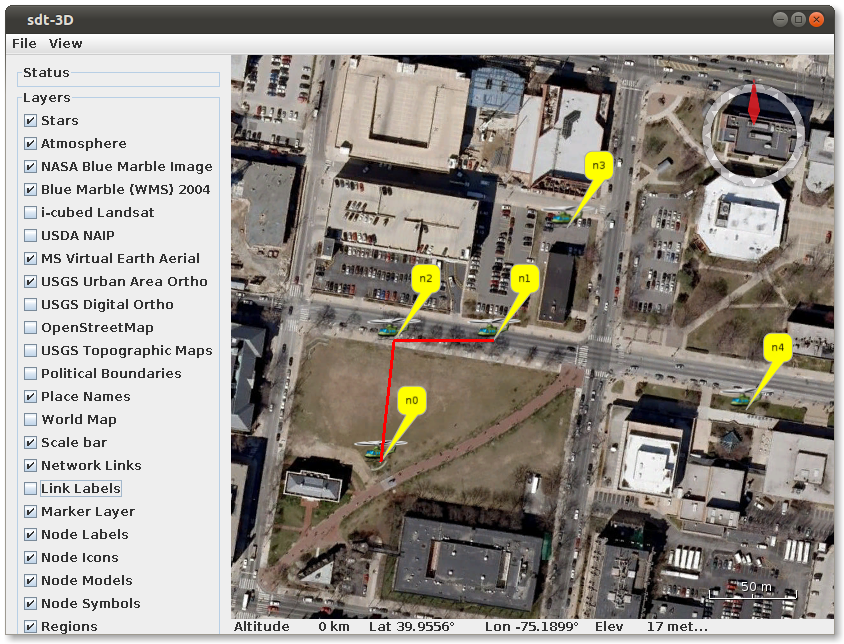
\includegraphics[scale=.3]{../prototype/images/ss2.png}
  \caption[A screenshot of the AHOY Display Tool (SDT)]%
  {The AHOY Display Tool (SDT) shows mobile nodes (represented by the helicopters) interacting on the world map.  The terrain (the city below) can
  also be seen.  The red lines between nodes represent a network connection.  Connected nodes become stationary as
  unconnected nodes continuosly change their position in the simulation until they come within range of another node.}
\end{figure}

\subsubsection{Visualization}
The following applies to AHOY's Visualization Engine (VE):
    \paragraph{Terrain} The Visualization Engine displays varying types of terrain, as defined by the environment.
    \paragraph{World Objects} The Visualization Engine displays mobile and static world objects, as defined by the scenario.
    \paragraph{Mobile Agents} The Visualization Engine displays mobile nodes.
    \paragraph{Path-finding} The Visualization Engine finds the path for an object to move to a given coordinate.
    \paragraph{Maximum Models} The Visualization Engine is able to display 300 models in a given scenario.
    \paragraph{Modularity} The Visualization Engine component is modular, i.e. it can be removed from the framework without affecting functionality (with the exception of the visuals).
    \paragraph{Timing} The Visualization Engine runs in real-time.
    \paragraph{Viewpoints} The Visualization Engine is able to display the world from more than one point of view.
    \paragraph{Viewpoints} The Visualization Engine is able to display the world from any given point of view.

\subsubsection{Simulation Engine}
	The following applies to AHOY's Simulation Engine (SE):
    \paragraph{Timing} The Simulation Engine runs in real-time.
    \paragraph{Limitations of Movement} The Simulation Engine limits the movement of models to specific areas or types of terrain (e.g. boats may only move on river).
    \paragraph{Path-drawing} The Simulation Engine finds the path for an object to move to a given coordinate.
    \paragraph{Collision Prevention} When finding a path, the Simulation Engine ensures the path will not steer an agent to navigate into world objects.
    \paragraph{Maximum Models} The Simulation Engine keeps in memory up to 300 nodes.
    \paragraph{User Intervention} The Simulation Engine allows for the interruption or change of events by human input.

\subsubsection{Network Definition}
	\paragraph{Interfaces} The definition language specifies interfaces on each virtual node.  Specifically, each interface is described with a physical model (radio, wired, etc.) and an appropriate link-layer protocol.
	\paragraph{Networks} The definition language specifies networks to which interfaces may interact.  Networks are described with a unique identifier and physical layer model (e.g. radio propagation model).
	\paragraph{Links} The definition language specifies one-to-one links between interfaces.  A link is	described by a physical layer model.

\subsubsection{Scenario Definition}
	\paragraph{Location} The scenario definition language defines the location of agent and non-agent world objects.
	\paragraph{Mobility} The scenario definition language describes the mobility or each virtual node as a function of time.
	\paragraph{Events} Mobility is alterable as a result of events, specified in the scenario definition.
	\paragraph{Non-node Behavior} The scenario definition language describes the movement of and events triggered by entities other than virtual nodes.

\subsubsection{Agent Framework}
	\paragraph{Agent Location} The agent framework specifies on which virtual node(s) a given agent should operate.
	\paragraph{Startup} The agent framework specifies the startup parameters of each agent.
	\paragraph{Collection} The agent framework specifies the output parameters of each agent instance.

\subsubsection{Distribution Framework}
	The Distribution Framework uses the API to spread the simulation across a Physical Distribution, and to aggregate trial data. It consists of a network of one-to-many physical machines.
	\paragraph{Physical Distribution} The distribution framework distributes virtual nodes evenly across physical nodes. Further, it handles the establishment and initialization of agents on their respective physical node.
	\paragraph{Simulation Server} The distribution framework organizes physical nodes hierarchically to interact with the simulation server.

\subsubsection{Data Aggregation}
    \paragraph{Real-Time Event Subscription} The simulator has an open API channel which should be used to monitor real-time events published by the simulation.

%___________________________________________________________________________

\subsubsection{Data Storage%
  \label{data-storage}%
}
    \paragraph{Outside Databases} No outside database system is used for data storage, unless it is introduced by the user via the API
    \paragraph{Scenario Definitions} Scenario definitions, including the topology and agents, are stored and parsed by the system

%___________________________________________________________________________

\subsection{Non-Functional Requirements} 
%___________________________________________________________________________

\subsubsection{Hardware Interfaces%
  \label{hardware-interfaces}%
}

AHOY requires that the machine running the system has one to many network interfaces to support distribution.

%___________________________________________________________________________

\subsubsection{Software Interfaces%
  \label{software-interfaces}%
}

AHOY requires the use of OpenGL in order to use the visualizer.

%___________________________________________________________________________

\subsubsection{Memory Constraints%
  \label{memory-constraints}%
}

AHOY requires a machine with at least 4GB of RAM.

%___________________________________________________________________________

\subsubsection{Site Adaptation Requirements%
  \label{site-adaptation-requirements}%
}

AHOY requires that the system is configured per-site to create a distributed simulation, or to interact on-the-fly.

%__________________________________________________________________________

\subsubsection{Operating System%
  \label{operating-system}%
}

AHOY is able to run on Unix, Linux, and Mac

%__________________________________________________________________________

\subsubsection{Processor% 
  \label{processor}%
}

AHOY requires at least a 32- or 64-bit x86 3.0GHz processor

%__________________________________________________________________________

\subsubsection{Network Connection%
  \label{network-connection}%
}

AHOY requires any recent network card which is currently connected to the simulation network (if the simulation is
distributed)

%__________________________________________________________________________

\subsubsection{Visualizer%
  \label{visualizer}%
}

AHOY requires a graphics card which will support OpenGL or an equivalent

%__________________________________________________________________________

\subsection{Input Formats%
  \label{input-formats}%
}

\subsubsection{Scenario}
    \paragraph{Location Data} The simulation is able to read location data for nodes.
	\paragraph{Mobility Data} The simulation is able to read mobility data for nodes.
	\paragraph{Scenario Input} The simulation is able to respond to event input from scenario input files

\subsubsection{Topology}
    \paragraph{Network Interfaces} The simulation is able to read network interfaces for nodes
    \paragraph{Network Links} The simulation is able to read links in the network between interfaces
    \paragraph{Network Topology} The simulation is able to read changes to the network topology

% NOTE: Believe we settled on no Network input.
%\subsubsection{Network}
%\begin{enumerate}
%		\item Nodes designated by the Topology shall be able to read in 802.11 (Wireless) traffic
%		\item Nodes designated by the Topology shall be able to read in TCP traffic
%		\item Nodes designated by the Topology shall be able to read in UDP traffic
%\end{enumerate}

%___________________________________________________________________________

\subsection{Output Formats%
  \label{output-formats}%
}
\subsubsection{Scenario}
    \paragraph{Network Changes} The system supports outputting network data changes over time post-simulation
    \paragraph{Network Fidelity} The system supports outputting network fidelity over time post-simulation

\subsubsection{Topology}
	\paragraph{Topology Changes} The system supports outputting topology changes over time post-simulation
	\paragraph{Mobility Patterns} The system supports outputting agent and non-agent mobility patterns post simulation

%___________________________________________________________________________

\subsection{User Interface%
  \label{user-interface}%
}

The following applies to AHOY's basic interface:
\subsubsection{Scenarios}
    \paragraph{Scenario} The interface allows a user to define a scenario.
    \paragraph{Scenario Language} The scenario defined by the interface is written in the Scenario Language.
\subsubsection{Experimentation}
    \paragraph{Beginning Experiment} The interface allows a user to begin an experiment.
    \paragraph{Ending Experiment} The interface allows a user to end an experiment.

%___________________________________________________________________________

\subsection{Extensibility%
  \label{extensibility}%
}
\subsubsection{Customization}
    \paragraph{Custom Topologies} The system provides a means for users to create custom topologies.
    \paragraph{Custom Agents} The system provides a means for users to create custom agents.

\subsection{Testing%
    \label{testing}%
}
All code with in the system must be tested. Core functionality of the software has 100\% code coverage with automated unit and integration tests.  The visualizer testing is done manually as it is a smaller component and would otherwise require a disproportionately large investment in initial setup.  Unit tests cover the algorithms used in our system while integration tests are used to test our data-flow.  

\section{System Evolution}

With more time, the AHOY team could create additional tools to aid in the the development of more complex agents or topologies, so that user customization does not become too granular.  Furthermore, tools which can automate or assist in data collection and parsing could be implements.  Even further development could lead to a platform that included Windows or other operating systems.

%___________________________________________________________________________

\subsection{Documentation%
  \label{documentation}%
}
\begin{enumerate}
    \item The software provides a User Manual containing step-by-step instructions for user perspective in Section~\ref{user-characteristics}.
    \item The software provides Developer Documentation containing:
    \begin{enumerate}
        \item Scenario Language syntax and usage
        \item Network Topology definitions and example networks
        \item Agent Framework definitions and example agents
    \end{enumerate}
\end{enumerate}

%___________________________________________________________________________

\appendix
\pagebreak

\end{document}
